
%%%%%%%%%%%%%%%%%%%%%%%%%%%%%%
%%%%%%%%%%%%%%%%%%%%%%%%%%%%%%
%%%%%%%%%%%%%%%%%%%%%%%%%%%%%%
%%%%%%%%%%%%%%%%%%%%%%%%%%%%%%
%%%%%%%%%%%%%%%%%%%%%%%%%%%%%%
%%%%%%%%%%%%%%%%%%%%%%%%%%%%%%
%%%%%%%%%%%%%%%%
%%%%%%%%%%%%%%%%
%%%%%%%%%%%%%%%%         CHAPTER 3
%%%%%%%%%%%%%%%%
%%%%%%%%%%%%%%%%
%%%%%%%%%%%%%%%%%%%%%%%%%%%%%%
%%%%%%%%%%%%%%%%%%%%%%%%%%%%%%
%%%%%%%%%%%%%%%%%%%%%%%%%%%%%%
%%%%%%%%%%%%%%%%%%%%%%%%%%%%%%
%%%%%%%%%%%%%%%%%%%%%%%%%%%%%%
%%%%%%%%%%%%%%%%%%%%%%%%%%%%%%




%%%%%%%%%%%%%%%%%%%%%%%%%%%%%%%%%%%%%%%%%%%%%%%%%%%%%%%%%%%%%%%%%%%%%%%%%%%%%%%%
\section{Insert a Figure}
\label{sec::ch3::problem-def}
Always make sure that figure file path in the code is consistent with where the file is located. The path assumes to start from the root of the LaTex folder. In the following example, the figure is in the sub-folder ``figures/examples''. It is always a good practice to organize your figures using multiple levels of folders.
\begin{figure}[!h]
\centering%
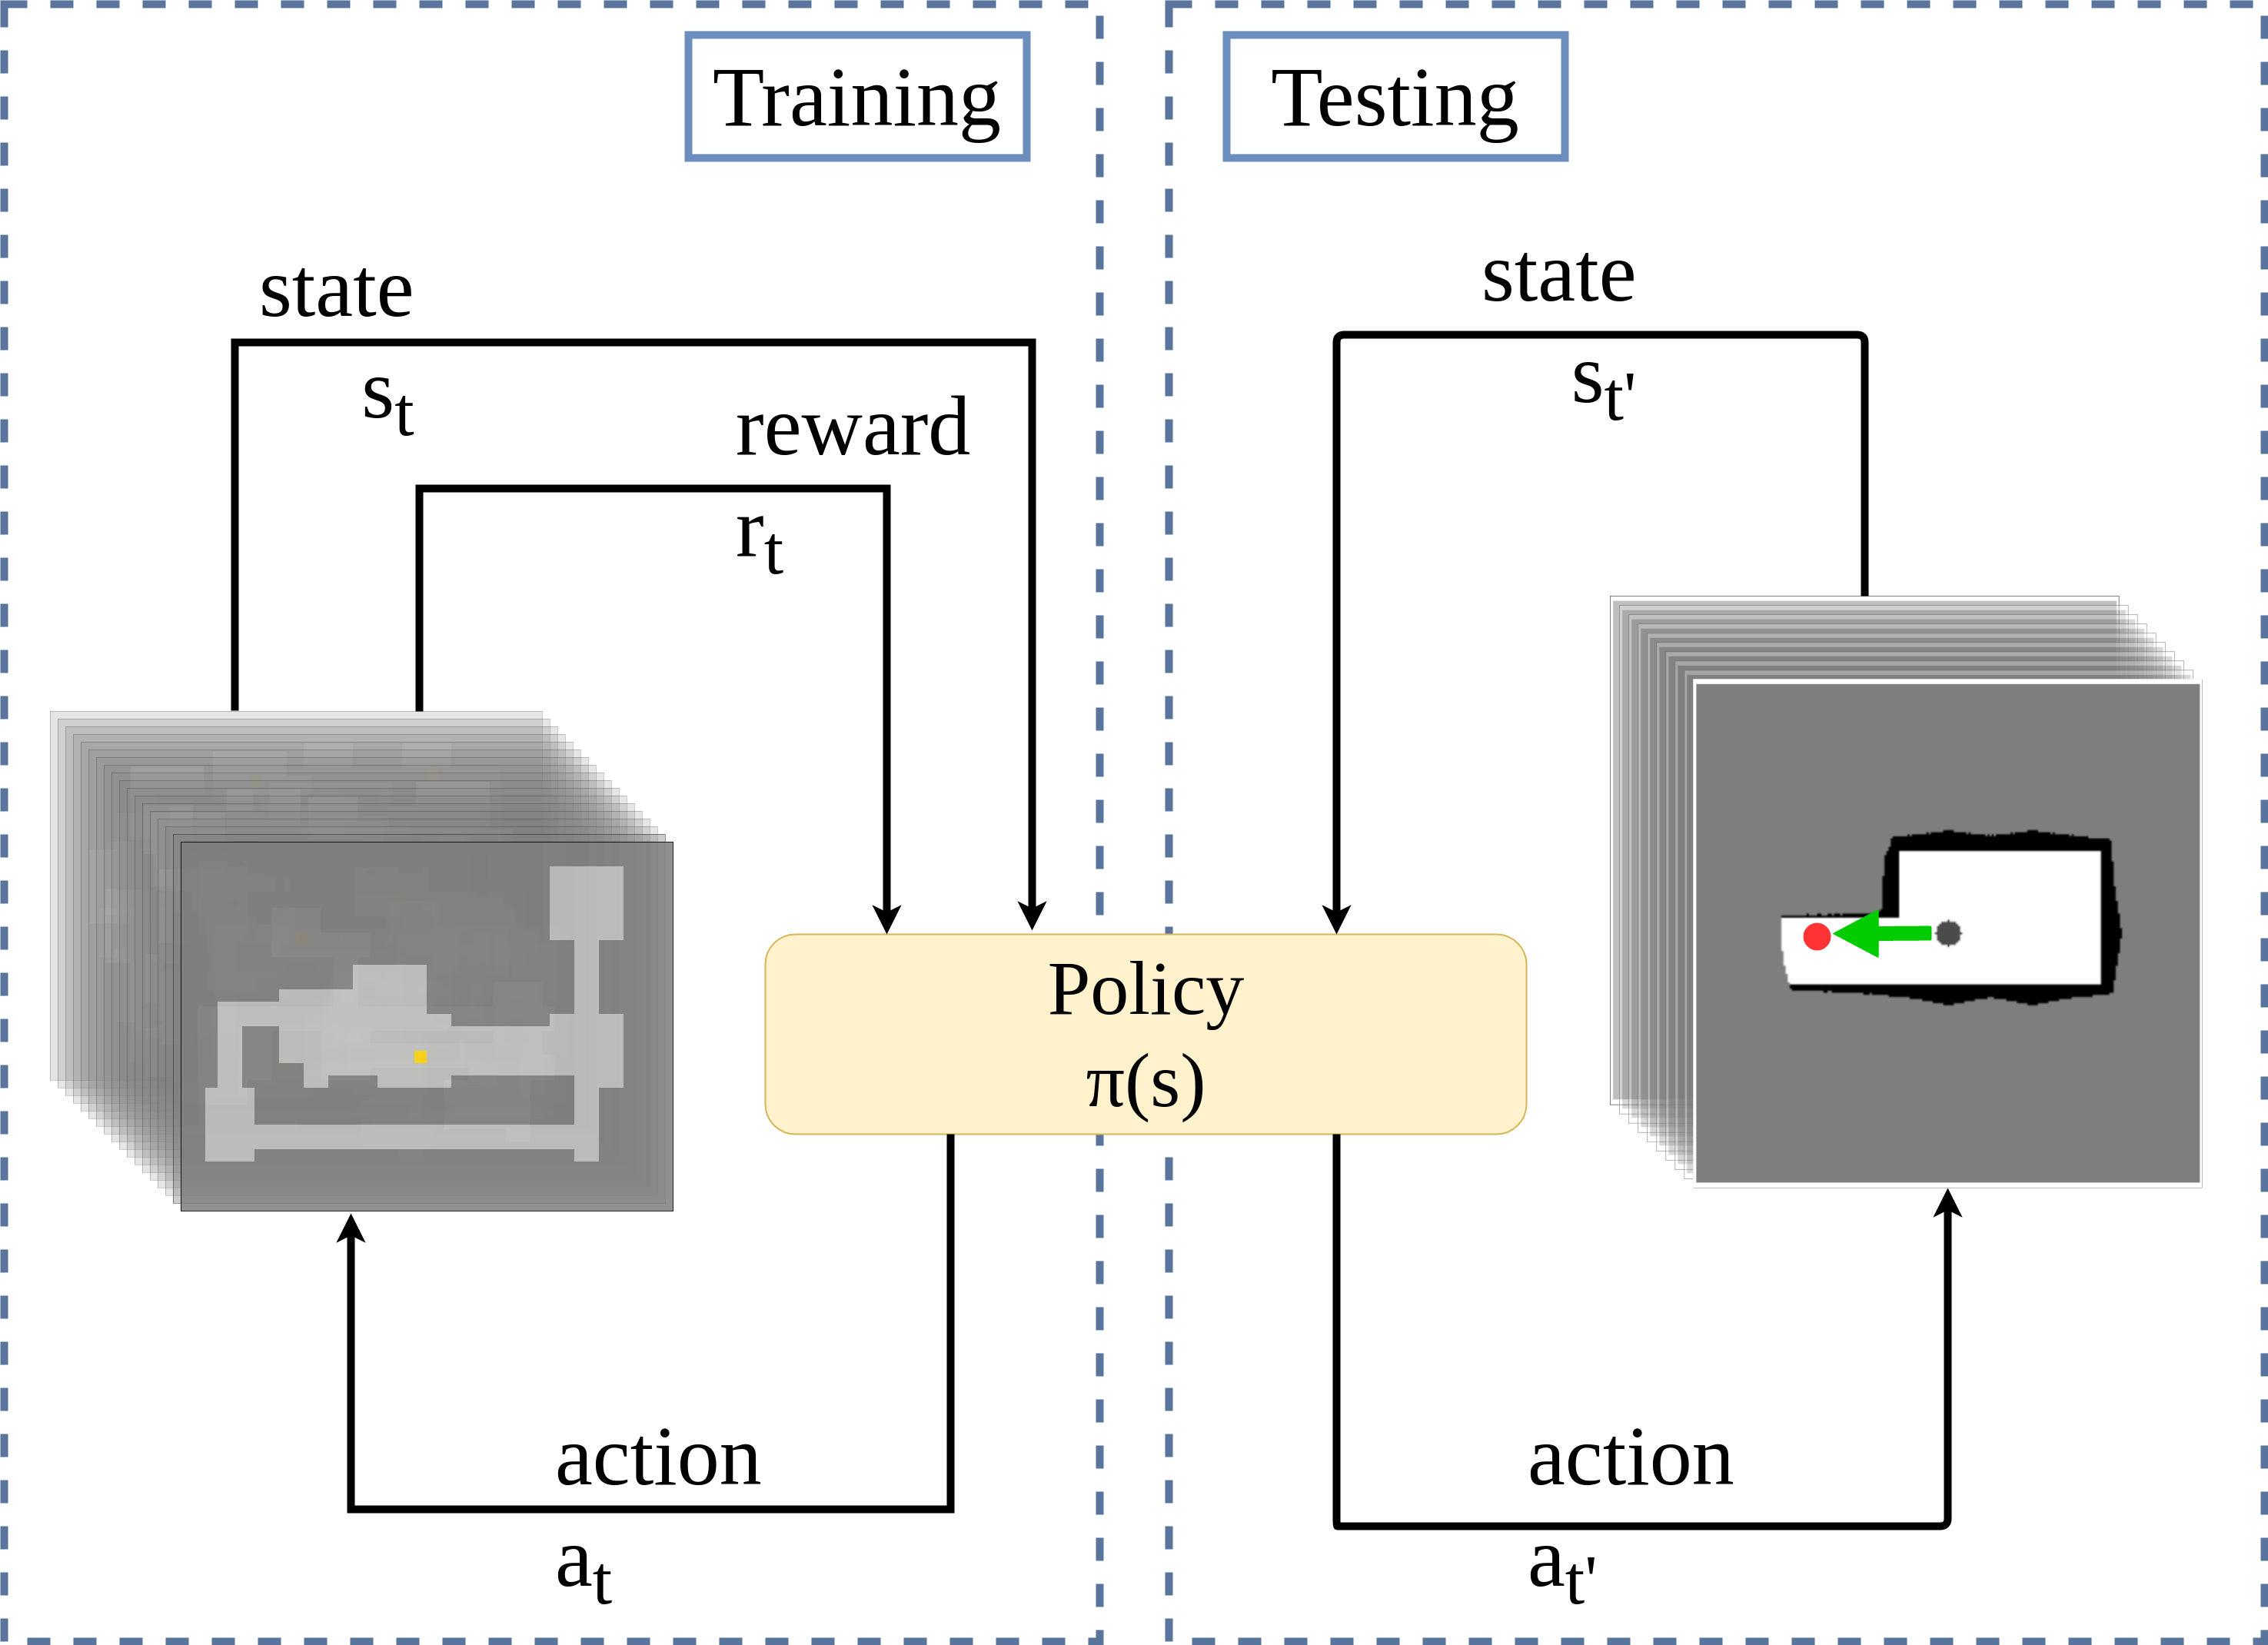
\includegraphics[width=0.49\columnwidth]{figures/examples/environments.png}
\caption{Always make sure to explain things in the capture}
\label{fig::ch3::environments}
\end{figure}

\lipsum[11-12]
%%%%%%%%%%%%%%%%%%%%%%
\clearpage